% -- Anfang Präambel
\documentclass[german,  % Standardmäßig deutsche Eigenarten, englisch -> english
parskip=full,  % Absätze durch Leerzeile trennen
%bibliography=totoc,  % Literatur im Inhaltsverzeichnis (ist unüblich)
%draft,  % TODO: Entwurfsmodus -> entfernen für endgültige Version
]{scrartcl}
\usepackage[utf8]{inputenc}  % Kodierung der Datei
\usepackage[T1]{fontenc}  % Vollen Umfang der Schriftzeichen
\usepackage[ngerman]{babel}  % Sprache auf Deutsch (neue Rechtschreibung)

% Mathematik und Größen
\usepackage{amsmath}
\usepackage[locale=DE,  % deutsche Eigenarten, englisch -> US
separate-uncertainty,  % Unsicherheiten seperat angeben (mit ±)
]{siunitx}
\usepackage{physics}  % Erstellung von Gleichungen vereinfachen
\usepackage{stmaryrd} %Widerspruchszeichen
\usepackage{amssymb}
\usepackage{graphicx}  % Bilder einbinden \includegraphics{Pfad/zur/Datei(ohne Dateiendung)}

% Gestaltung
%\usepackage{microtype}  % Mikrotypographie (kann man am Ende verwenden)
\usepackage{booktabs}  % schönere Tabellen
%\usepackage[toc]{multitoc}  % mehrspaltiges Inhaltsverzeichnis
\usepackage{csquotes}  % Anführungszeichen mit \enquote
\usepackage{caption}  % Anpassung der Bildunterschriften, Tabellenüberschriften
\usepackage{subcaption}  % Unterabbildungen, Untertabellen, …
\usepackage{enumitem}  % Listen anpassen
\setlist{itemsep=-10pt}  % Abstände zwischen Listenpunkten verringern

% Manipulation des Seitenstils
\usepackage{scrpage2}
% Kopf-/Fußzeilen setzen
\pagestyle{scrheadings}  % Stil für die Seite setzen
\clearscrheadings  % Stil zurücksetzen, um ihn neu zu definieren
\automark{section}  % Abschnittsnamen als Seitenbeschriftung verwenden
\ofoot{\pagemark}  % Seitenzahl außen in Fußzeile
\ihead{\headmark}  % Seitenbeschriftung mittig in Kopfzeile
\setheadsepline{.5pt}  % Kopzeile durch Linie abtrennen

\usepackage[hidelinks]{hyperref}  % Links und weitere PDF-Features

% TODO: Titel und Autor, … festlegen
\newcommand*{\titel}{Magneto-Widerstandseffekte in dünnen magnetischen Schichten}
\newcommand*{\autor}{Tom Drechsler, Konstantin Schmid}
\newcommand*{\abk}{MR}
\newcommand*{\betreuer}{Richard Schlitz}
\newcommand*{\messung}{19. Dezember 2019}
\newcommand*{\ort}{REC/D008}

\hypersetup{pdfauthor={\autor}, pdftitle={\titel}}  % PDF-Metadaten setzen




% Subsubsubsection erzeugen
\usepackage{titlesec}
\usepackage{hyperref}

\titleclass{\subsubsubsection}{straight}[\subsection]

\newcounter{subsubsubsection}[subsubsection]
\renewcommand\thesubsubsubsection{\thesubsubsection.\arabic{subsubsubsection}}
\renewcommand\theparagraph{\thesubsubsubsection.\arabic{paragraph}} % optional; useful if paragraphs are to be numbered

\titleformat{\subsubsubsection}
  {\normalfont\normalsize\bfseries}{\thesubsubsubsection}{1em}{}
\titlespacing*{\subsubsubsection}
{0pt}{3.25ex plus 1ex minus .2ex}{1.5ex plus .2ex}

\makeatletter
\renewcommand\paragraph{\@startsection{paragraph}{5}{\z@}%
  {3.25ex \@plus1ex \@minus.2ex}%
  {-1em}%
  {\normalfont\normalsize\bfseries}}
\renewcommand\subparagraph{\@startsection{subparagraph}{6}{\parindent}%
  {3.25ex \@plus1ex \@minus .2ex}%
  {-1em}%
  {\normalfont\normalsize\bfseries}}
\def\toclevel@subsubsubsection{4}
\def\toclevel@paragraph{5}
\def\toclevel@paragraph{6}
\def\l@subsubsubsection{\@dottedtocline{4}{7em}{4em}}
\def\l@paragraph{\@dottedtocline{5}{10em}{5em}}
\def\l@subparagraph{\@dottedtocline{6}{14em}{6em}}
\makeatother

\setcounter{secnumdepth}{4}
\setcounter{tocdepth}{4}


\addto{\captionsngerman}{
\renewcommand*{\figurename}{Abb.}
}                   % Ändern der Grafikbeschriftung von "Abbildung:" zu "Abb.:"



% automatischen Titel konfigurieren
\titlehead{F-Praktikum \abk \hfill TU Dresden}
%\subject{Interferometer}
\title{\titel}
\author{\autor}
\date{\begin{tabular}{ll}
Protokoll: & \today\\
Messung: & \messung\\
Ort: & \ort\\
Betreuer: & \betreuer\end{tabular}}

% -- Ende Präambel

\begin{document}
\begin{titlepage}
\maketitle  % Titel setzen
\tableofcontents  % Inhaltsverzeichnis setzen
\end{titlepage}

\section{Ziel und Versuchsprinzip}
Der Magnetwiderstand ist eine besondere Eigenschaft einiger Materialien und Heterostrukturen, ihren elektrischen Widerstand unter Anwesenheit eines externen Magnetfeldes zu ändern. Dazu gehören verschiedene Effekte, die unterschiedliche Ursachen und Ausprägungen haben. In diesem Versuch sollen ausgewählte magnetoresistive Effekte untersucht und deren technische Anwendung diskutiert werden. Dazu gehören insbesondere das Verhalten von Materialien in Abhängigkeit von der Stärke und der Richtung des äußeren Feldes.
\section{Theoretische Grundlagen}
Es gibt eine recht große Fülle an verschiedenen Phänomenen, die man unter dem Begriff magnetoresistive Effekte zusammenfasst. Im folgenden sollen zunächst die wichtigsten Begriffe zur Beschreibung des Magnetismus in Materie knapp dargestellt werden. Es folgt eine Übersicht zu den hier untersuchten magnetoresisitiven Effekten. Diese umfasst den Hall-Effekt, den anisotropen Magnetwiderstand sowie den Riesenmagnetwiderstand.
\subsection{Magnetismus - Grundlagen}
Dieser Abschnitt dient im wesentlichen der Zusammenstellung von Grundgleichungen und Begriffen, insbesondere im Hinblick auf das verwendete Einheitensystem. Zusätzlich erfolgt eine kurze Darstellung der magnetischen Hysterese.
\subsubsection{Begriffe der Elektrodynamik in Materie}
Die klassische Theorie des Elektromagnetismus wird durch die mikroskopischen Maxwell-Gleichungen exakt beschrieben. Sie erlauben die Berechnung von Feldern aus gegebenen Ladungs- und Stromverteilung sowie das Aufstellen von Bewegungsgleichungen für geladenen Teilchen in vorgegebenen Feldern. Diese Gleichungen haben allerdings den Nachteil, dass sie für jede Beschreibung von elektromagnetischen Phänomenen in Materie ungeeignet sind, weil man sowohl den Zustand als auch das Feld jedes einzelnen Teilchens des betrachteten Materiestücks benötigen würde. Um dennoch eine brauchbare Theorie zu entwickeln, wird eine räumliche Mittelung der Materie durchgeführt. Diese bildet dann das kollektive Verhalten des gesamten Stücks Materie ab und ist einer experimentellen Überprüfung damit auch angemessener. Um die Rechnung einfacher zu gestalten, trennt man zusätzlich gedanklich die felderzeugenden (sog. freien) Ladungen und Ströme von denen, die in der Materie induziert werden. Entsprechend werden auch die Felder zerlegt in ein äußeres Feld und eine Antwort des Systems. Man erhält dabei einerseits die makroskopischen Maxwell-Gleichungen
\begin{align*}
\vec{\nabla}\cdot\vec{D}(\vec{r},t) &= \rho_{\mathrm{frei}}(\vec{r},t)   && \vec{\nabla}\cdot\vec{B}(\vec{r},t) = 0 \\
\vec{\nabla}\times\vec{E}(\vec{r},t) &= -\frac{\partial}{\partial t}\vec{B}(\vec{r},t)    &&\vec{\nabla}\times\vec{H}(\vec{r},t) = \vec{j}_{\mathrm{frei}}(\vec{r},t) + \frac{\partial}{\partial t}\vec{D}(\vec{r},t) 
\end{align*}
und andererseits die Materialgleichungen für die Hilfsfelder der dielektrischen Verschiebung \(\vec{D}\) und der magnetischen Feldstärke \(\vec{H}\):
\begin{align*}
\vec{D} = \varepsilon_0 \vec{E} + \vec{P} \quad\quad \vec{H} = \frac{1}{\mu_0}\vec{B} - \vec{M}
\end{align*}
Dabei bezeichnen \(\vec{P}\) die Polarisation und \(\vec{M}\) die Magnetisierung, welche die Antwort der Materie auf äußere Felder beschreiben. Sie lassen sich nicht allein aus der Elektrodynamik ableiten, sondern benötigen i.Allg. eine mikroskopische Theorie, die Ergebnisse der Quantenmechanik und der Atom- und Molekülphysik umfasst. 
\subsubsection{Magnetische Permeabilität und Arten des Magnetismus}
Um die Reaktion der Materie auf externe Magnetfelder zu beschreiben, geht man von \(\vec{B} = \mu_0(\vec{H} + \vec{M}) = \vec{B}(\vec{H})\) aus, d.h. man betrachtet die fundamentale Größe der magnetischen Flussdichte als Funktion von \(\vec{H}\). Ein allgemeiner Ansatz für den funktionalen Zusammenhang ist
\[B_i = \sum_{j}\mu_{ij}^{(1)} H_{j} + \sum_{k}\sum_{j}\mu_{ijk}^{(2)} H_{j}H_k  + \hdots\]
Die Größen \(\mu_{ij}^{(1)},\mu_{ijk}^{(2)},\hdots\) sind dabei Tensoren zweiter, dritter und höherer Stufe. Der Tensorcharakter bringt die Anisotropie zum Ausdruck, da i.Allg. die Vektoren \(\vec{B}\) und \(\vec{H}\) nicht parallel liegen und kristalline Stoffe idR. ausgezeichnete Richtungen haben. Beschränkt man sich auf den ersten Summanden, so ergibt sich ein linearer Zusammenhang zwischen \(\vec{B}\) und \(\vec{H}\). Die übrigen Terme enthalten eine Kopplung zwischen den verschiedenen Komponenten von \(\vec{H}\) und sind damit nichtlinear. Die Behandlung der Nichtlinearität ist ungleich schwieriger, eröffnet aber die Beschreibung vieler interessanter Phänomene. In dieser Arbeit beschränken wir uns ausschließlich auf den Fall linearer Zusammenhänge. Die Antwort des Systems auf externe Felder erlaubt eine einfache Einteilung der magnetischen Materialien in folgende wichtigste Klassen:
\begin{enumerate}
\item Falls die Materie ohne externes Feld schon ungeordnete magnetische Dipole enthält, werden diese unter dem Einfluss eines Feldes ausgerichtet. Innerhalb des Stoffes kommt es damit zu einer Verstärkung des Magnetfeldes. Solche Stoffe heißen \textbf{paramagnetisch}.
\item Es ist aber auch möglich, dass im Material bereits magnetische Dipole vorhanden sein, die sich teilweise parallel ausgerichtet haben. Sie bilden sogenannte Weiss'sche Bezirke, wobei innerhalb eines Bezirks eine vollständige Ausrichtung vorliegt. Die verschiedenen Bezirke sind bloß unterschiedlich gegeneinander orientiert. Beim Anlegen eines externen Feldes verstärken diese Materialien das Feld um ein Vielfaches (bis 500.000fach). Da dieser Effekt besonders bei Eisen, Nickel und Cobalt auftritt, nennt man solche Materialien \textbf{ferromagnetisch}. 
\item Falls die Materie noch keine magnetischen Dipole enthält, werden diese durch ein externes Feld erst erzeugt. Innerhalb des Stoffes zeigt die Magnetisierung dann entgegen dem äußeren Feld, sodass das Magnetfeld dort geschwächt wird. Derartige Materialien heißen \textbf{diamagnetisch}. Eine Sonderrolle nehmen hierbei die Supraleiter 1. Art ein. Diese bilden bei Kühlung unter die Sprungtemperatur einen idealen Diamagneten, d.h. das Feld wird vollständig aus dem Inneren der Probe verdrängt (Meißner-Ochsenfeld-Effekt).
\end{enumerate}
Daneben gibt es noch eine feinere Unterteilung hinsichtlich der Beiträge zum Magnetismus (Pauli-Paramagnetismus, Langevin-Diamagnetismus,\(\hdots\)), sowie zahlreiche weitere Phänomene (z.B. Antiferromagnetismus). Für diesen Versuch ist diese einfache Einteilung aber ausreichend.
\subsubsection{Magnetische Hysterese}
Bringt man ein anfangs unmagnetisches ferromagnetisches Material in ein externes Feld und untersucht \(B = |\vec{B}|\) im Festkörper in Abhängigkeit vom externen Feld \(H = |\vec{H}|\), so kann man schrittweise die folgenden Prozesse beobachten:
\begin{figure}[h!]\centering
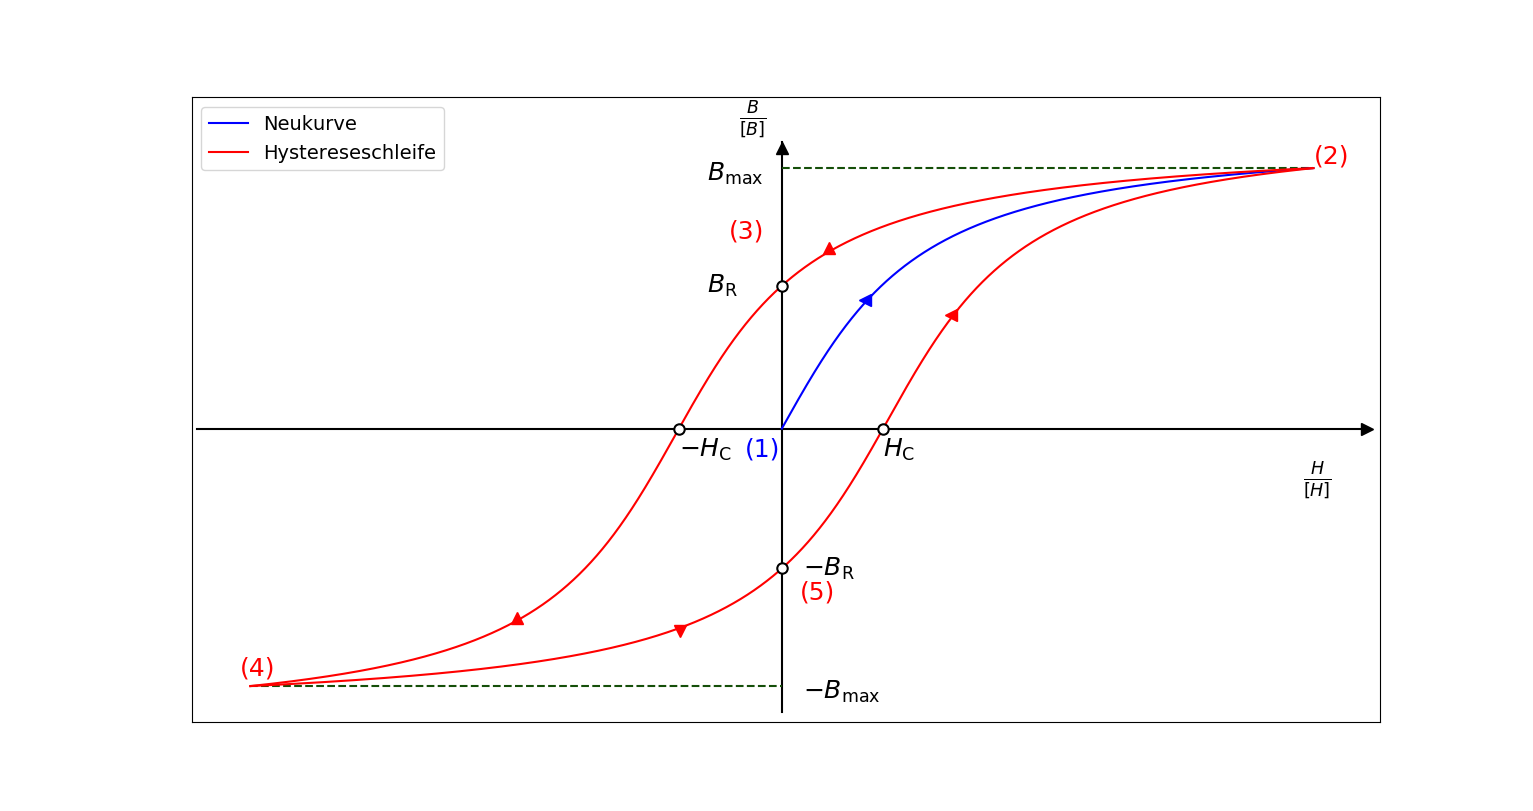
\includegraphics[width=\textwidth]{Hysteresekurve.png}
\caption{Illustration des typischen Hystereseverhaltens \(B(H)\) einer ferromagnetischen Probe im externen Feld \(H\)}
\end{figure}
\newpage
\begin{itemize}
\item \(1\rightarrow 2\): Mit steigendem externen Feld \(H\) erhöht sich auch \(B\) von null bis zur Sättigung \(B_{\mathrm{max}}\). Die hierbei entstehende Kurve heißt Neukurve.
\item \(2\rightarrow 3\): Nach Abschalten des Feldes auf \(H=0\) behält das Material eine positive Restmagnetisierung, die sogenannte Remanenz \(B_{\mathrm{R}}\). 
\item \(3\rightarrow 4\) Bei Umkehr des externen Feld \(H\) wird zuerst die Remanenz aufgehoben; der dafür notwendige Wert von \(H\) heißt Koerzitivfeldstärke \(-H_{\mathrm{C}}\). Anschließend wechselt \(B\) das Vorzeichen und nimmt wieder einen Sättigungswert \(-B_{\mathrm{max}}\) an.
\item \(4\rightarrow 5\) Beim erneuten Abschalten des Feldes \(H\) verbleibt wieder eine Restmagnetisierung. Die Remanenz \(-B_{\mathrm{R}}\) ist diesmal allerding negativ. 
\item \(5\rightarrow 2\) Bei Erhöhung von \(H\) wird abermals erst die Remanenz durch die Koerzitivfeldstärke \(H_{\mathrm{C}}\) aufgehoben. Anschließend steigt \(B\) wieder bis zu Sättigung.
\end{itemize}
Die rote Kurve wird danach erneut umlaufen. Die Neukurve beschreibt dabei nur die erstmalige Magnetisierung und kann durch Ummagnetisieren i.Allg. nicht mehr erreicht werden, sondern nur durch zerstören der ferromagnetischen Ordnung durch starkes Erhitzen. Die Magnetisierung eines Materials ist damit nicht nur vom externen Feld \(H\) allein, sondern auch mehr oder weniger empfindlich von der Vorbehandlung des Materials abhängig. Dieses Phänomen wird als \textbf{magnetische Hysterese} bezeichnet. Die von der Hysteresekurve umschlossene Fläche ist ein Maß für die Verluste, die sich durch Ummagnetisierung ergeben. Anhand der Hysterese lassen sich die Werkstoffe einteilen in
\begin{itemize}
\item \underline{weichmagnetisches Material:} kleine Koerzitivfeldstärke und damit leicht ummagnetisierbar, sehr schlanke und deutlich s-förmige Hysteresekurve
\item \underline{hartmagnetisches Material:} hohe Koerzitivfeldstärke und damit schwer ummagnetisierbar, sehr breite und nahezu rechteckige Hysteresekurve
\end{itemize}
In der folgenden Abbildung sind typische Hystereskurven hart- und weichmagnetischer Werkstoffe gegenübergestellt:
\subsection{Magnetoresistive Effekte}
Im folgenden werden die für diesen Versuch bedeutsamen Magnetowiderstandseffekte erläutert. Diese sind der Hall-Effekt, der Anisotrope Magnetwiderstand und der Riesenmagnetwiderstand.
\subsubsection{Der Hall-Effekt}
Hierbei handelt es sich um ein Transportphänomen, dass der Physiker Edwin \textsc{Hall} 1879 in seiner Doktorarbeit nachgewiesen hat. Der Effekt kann bereits klassisch verstanden werden: Wird ein stromdurchflossener Leiter in ein Magnetfeld gebracht, wirkt auf die Elektronen die Lorentzkraft \(\vec{F} = e\vec{v}\times\vec{B}\). Das Magnetfeld führt dabei zu einer seitlichen Driftbewegung der Elektronen senkrecht zur Stromrichtung. Dadurch baut sich senkrecht zur Stromrichtung ein elektrisches Feld auf, welches nach kurzer Zeit die Driftbewegung kompensiert. Das elektrische Feld äußert sich in einer zusätzlichen Spannung senkrecht zur Stromrichtung, der \textbf{Hall-Spannung}. Für diese erhält man durch einfache Rechnung
\[U_{\mathrm{H}} = R_{\mathrm{H}}\cdot\frac{BI}{d}\]
wobei \(B\) die magnetische Flussdichte, \(I\) die Stromstärke und \(d\) die Dicke der Probe in Feldrichtung ist. Die Hall-Konstante \(R_{\mathrm{H}}\) ist ein Materialparameter und lässt sich für viele einfache Materialien mit nur einem Leitungsband durch \(R_{\mathrm{H}} = -\frac{1}{nq}\) berechnen, wobei \(q\) die Ladung (mit Vorzeichen!) und \(n\) die Ladungsträgerdichte ist. Der Hall-Effekt lässt sich vielfältig anwenden:
\begin{itemize}
\item Bei bekannter Hall-Konstante kann man mit einer Hall-Sonde ein sehr einfach zu bauendes Messgerät für Magnetfelder realisieren. 
\item Durch ein bekanntes Magnetfeld kann man umgekehrt die Hall-Konstante bestimmen. Sie erlaubt dann Rückschlüsse auf die sonst schwer zugängliche Ladungsträgerdichte sowie das Vorzeichen der dominierenden Ladung. Dies ist insbesondere in der Halbleitertechnik unentbehrlich.
\end{itemize}
Der Vollständigkeit halber sei erwähnt, dass man den Hall-Effekt auch aus der linearisierten Boltzmann-Transportgleichung gewinnen kann. Eine zusätzliche Behandlung der quantenmechanischen Effekte im Festkörper ergibt dann zusätzlich eine ganze Reihe weiterer verwandter Phänomene, wie etwa den Quanten-Hall-Effekt, Righi-Leduc-Effekt und weitere.
\subsubsection{Der Anisotrope Magnetwiderstand (AMR)}
Der Anisotrope Magnetwiderstand (engl.: anisotropic magnetic resistance, kurz AMR) war historisch gesehen der erste magnetoresistive Effekt, der entdeckt wurde. William \textsc{Thomson} beschrieb ihn bereits 1857. Wie der Name schon sagt, rührt dieser Effekt von der Anisotropie bestimmter Materialien her: Bei betragsmäßig konstanter Magnetisierung des Materials ergibt sich eine Abhängigkeit des elektrischen Widerstandes vom Winkel zwischen Magnetisierung und Strom gemäß
\[R = R_{\parallel} - (R_{\parallel} - R_{\perp})\sin^2\alpha\quad\text{mit}\quad \alpha = \sphericalangle (\vec{j},\vec{M})\in\left[-\frac{\pi}{2},\frac{\pi}{2}\right]\]
Dabei ist \(R_{\parallel}\) der Widerstand für \(\alpha=0\), d.h. \(\vec{j}\parallel\vec{M}\) und \(R_{\perp}\) der Widerstand für \(\alpha=\pm\frac{\pi}{2}\), d.h. \(\vec{j}\perp\vec{M}\).
Diese Abhängigkeit vom Winkel kann dadurch verstanden werden, dass nicht-kugelsymmetrische Orbitale wie z.B. die 3d-Orbitale durch die Magnetisierung eine Drehung erfahren. Dadurch ändert sich der Streuquerschnitt von Ladungen am Atom beim Durchgang durch den Leiter je nach Orientierung der Orbitale relativ zum Strom und somit auch der elektrische Widerstand. Die Größe des Anisotropen Magnetwiderstandes ist üblicherweise definiert durch
\[\frac{\Delta R}{R} := \frac{R_{\parallel} - R_{\perp}}{R_{\parallel}}\]
Oft gibt man diesen Wert auch prozentual an, indem man noch mit 100 multipliziert. Der AMR tritt bei vielen ferromagnetischen Materialien in Dünnschichten auf und liegt größenordnungsmäßig bei etwa \(\frac{\Delta R}{R} \sim 1\hdots 4\%\).
\subsubsection{Der Riesenmagnetwiderstand (GMR)}
Beim Riesenmagnetwiderstand (engl.: giant magnetic resistance, kurz GMR) handelt es sich um ein relativ neues Phänomen, das 1988 von Peter \textsc{Grünberg} und Albert \textsc{Fert} entdeckt wurde. Der Effekt tritt in sogenannten Heterostrukturen auf, bei denen dünne ferromagnetische Schichten und nichtmagnetische Schichten immer abwechselnd übereinander gestapelt werden. Die ferromagnetischen Schichten können dabei eine parallele oder eine antiparallele Magnetisierung haben. Es zeigt sich nun, dass ein Elektron beim Übergang von einer Schicht in die nächste unterschiedlich gestreut wird, je nachdem wie sein Spin relativ zur Magnetisierung der Schicht steht. Man kann nun folgende zwei Fälle unterscheiden:
\begin{itemize}
\item Angenommen die Schichten sind parallel magnetisiert. Wenn sich ein Elektron in einer der Schichten gut ausbreiten kann, weil sein Spin günstig eingestellt ist, dann kann es das auch in der anderen Schicht. Wenn der Spin dagegen ungünstig eingestellt ist und es sich schlecht in der ersten Schicht ausbreiten kann, so gilt das auch für die zweite.
\item Wenn die Schichten dagegen antiparallel magnetisiert sind, dann ist es egal wie der Spin des Elektrons eingestellt ist, weil es entweder an der ersten oder an der zweiten Schicht stark gestreut wird.
\end{itemize}
Durch den zusätzlichen Spin-Freiheitsgrad erhält man also zwei Sorten Ladungsträger, nämlich Elektronen mit \(s=+\frac{1}{2}\) und Elektronen mit \(s= -\frac{1}{2}\). Da die Magnetisierung unmittelbar mit einer Vorzugsrichtung der Spins verknüpft ist, liegen die beiden Arten nicht gleich häufig vor. Die häufigere Art nennt man \textbf{Majoritätsladungsträger}, die weniger häufigere Art entsprechend \textbf{Minoritätsladungsträger}. Die Überlegung hat nun gezeigt, dass bei antiparalleler Magnetisierung der Schichten beide den gleichen Widerstand haben, bei paralleler Magnetisierung dagegen nicht. \\\\
Zur mathematischen Beschreibung stellt man sich nun vor, dass die Majoritäts- und die Minoritätsladungsträger jeweils einen eigenen Kanal bilden, da ja beide potentiell verschiedene Widerstände \(R_{\mathrm{maj}}\) und \(R_{\mathrm{min}}\) haben. Der gesamte Ladungstransport kann dann verstanden werden als eine Parallelschaltung der beiden Kanäle. Da für die Parallelschaltung zweier Widerstände gemäß den Kirchhoff'schen Regeln
\[\frac{1}{R_{\mathrm{ges}}} = \frac{1}{R_1} + \frac{1}{R_2} \quad\Longrightarrow\quad R_{\mathrm{ges}} = \frac{R_1 R_2}{R_1 + R_2}\]
gilt, erhält man im Einzelnen
\begin{align*}
\underline{\underline{R_{\mathrm{ges}}^{\mathrm{par}} = \frac{2R_{\mathrm{maj}} R_{\mathrm{min}}}{R_{\mathrm{maj}} + R_{\mathrm{min}}}  }} \quad\quad \underline{\underline{R_{\mathrm{ges}}^{\mathrm{anti}} = \frac{R_{\mathrm{maj}} + R_{\mathrm{min}}}{2}   }}
\end{align*}
Im Falle der parallelen Magnetisierung kann man zusätzlich die Annahme machen, dass \(R_{\mathrm{min}} \gg R_{\mathrm{maj}}\). Dadurch vereinfachen sich die Formeln nochmal:
\begin{align*}
\underline{\underline{R_{\mathrm{ges}}^{\mathrm{par}}  \approx 2R_{\mathrm{maj}} }} \quad\quad \underline{\underline{R_{\mathrm{ges}}^{\mathrm{anti}} = \frac{R_{\mathrm{min}}}{2}}  }
\end{align*}
Damit ist der Gesamtwiderstand bei paralleler Magnetisierung der Schichten deutlich kleiner als bei antiparalleler Magnetisierung. Mithilfe des GMR-Effektes kann man nun zwei interssante Anordnungen realisieren:
\begin{itemize}
\item Wenn die nicht-magnetische Trennschicht sehr dünn ist (ca. 1nm), können die ferromagnetischen Schichten miteinander wechselwirken. Es stellt sich dann von selbst eine relative Orientierung der Magnetisierungen zueinander ein. Über die Dicke der Trennschicht kann man einerseits die Stärke der Kopplung einstellen und andererseits festlegen, ob die parallele oder die antiparallele Orientierung energetisch bevorzugt wird. 
\item Verwendet man eine etwas dickere Schicht (ca. 3nm), gibt es keine nennenswerte Wechselwirkung mehr zwischen den Schichten. Eine solche Anordnung heißt auch \textbf{Spinventil}.
\end{itemize}
Insbesondere das Spinventil hat eine bemerkenswerte Eigenschaft: Verwendet man zwei verschiedene Materialien für die ferromagnetische Schicht, haben diese auch unterschiedliches Hystereseverhalten. Der weichmagnetische Stoff wird dann im externen Feld zuerst ummagnetisiert und der hartmagnetische erst bei einer höheren Feldstärke. Da die Schichten im Spinventil nicht wechselwirken, kann man so durch das externe Feld steuern, ob die Schichten parallel oder antiparallel magnetisiert sind und damit den Widerstand zwischen zwei Werten ändern. Das macht man sich in Festplatten zunutze. \\\\
Die Größe des GMR definiert man ähnlich wie schon beim AMR über das Verhältnis:
\[\frac{\Delta R}{R} = \frac{R_{\mathrm{ges}}^{\mathrm{par}} - R_{\mathrm{ges}}^{\mathrm{anti}}}{R_{\mathrm{ges}}^{\mathrm{anti}}}\]
Im Gegensatz zum AMR liegt die Größe des Riesenmagnetwiderstandes jedoch bei etwa \(\frac{\Delta R}{R}\sim 10\hdots 100\%\), daher auch der Name.
\section{Durchführung}
Im Folgenden soll zunächst die verwendete Messmethode erläutert sowie der Versuchsaufbau gezeigt werden. Es folgt eine Beschreibung der durchgeführten Messungen sowie der dabei aufgetretenen Beobachtungen und Besonderheiten.
\subsection{Zur Widerstandsmessung}
Für die Messung von Widerständen existieren zahlreiche verschiedene Experimentieranordnungen. Die Auswahl richtet sich idR. nach der geforderten Präzision an das Messergebnis sowie insbesondere an die Größe und eventuell die Art des Widerstandes. Für die Messung an der dünnen Schicht wurde eine sogenannte Vierpunktmessung verwendet, die wie folgt funktioniert:
\begin{enumerate}
\item Auf der zu untersuchenden dünnen Schicht werden an den Ecken vier Kontaktspitzen mit Leitsilber aufgebracht, die mit A,B,C und D durchnummeriert werden.
\item Zwichen den Kontakten A und B wird ein definierter Strom eingeprägt. Das Messgerät ermittelt die zwischen den Kontakten C und D abfallende Spannung und errechnet einen Wert 
\[R_{\mathrm{AB|CD}} = \frac{U_{\mathrm{CD}}}{I_{\mathrm{AB}}}\]
\item In einem zweiten Schritt wird das Verfahren nochmal mit zyklischer Vertauschung der Kontakte durchgeführt. Diesmal wird zwischen den Kontakten B und C ein definierter Strom eingeprägt sowie die zwischen D und A abfallende Spannung gemessen. Daraus wird dann ein weiterer Wert errechnet:
\[R_{\mathrm{BC|DA}} = \frac{U_{\mathrm{DA}}}{I_{\mathrm{BC}}}\]
\item Aus den beiden Werten wird der Widerstand errechnet.
\end{enumerate}
Die hier beschriebene Methode geht auf den holländischen Physiker Leo \textsc{van der Pauw} zurück, der sie 1958 entdeckte. Er bewies mit Methoden der Funktionentheorie, dass zwischen den beiden errechneten Widerständen \(R_{\mathrm{AB|CD}}\) und \(R_{\mathrm{BC|DA}}\), der Schichtdicke \(d\) und dem spezifischen elektrischen Widerstand \(\rho\) stets der Zusammenhang
\[\mathrm{exp}\left(-\frac{\pi d}{\rho}\cdot R_{\mathrm{AB|CD}}\right) + \mathrm{exp}\left(-\frac{\pi d}{\rho}\cdot R_{\mathrm{BC|DA}}\right) = 1\]
besteht und zwar unabhängig von der Form der dünnen Schicht und auch unabhängig von der Position der Kontakte, solange diese am Rand der Probe liegen. Die Formel ist außer für hochsymmetrische Formen nicht analytisch nach \(\rho\) lösbar, dafür aber numerisch mit beliebiger Genauigkeit. Man kann weiter zeigen, dass sich für Proben mit mindestens einer Symmetrieachse (z.B. rechteckige Folien) wegen \(R_{\mathrm{AB|CD}} \equiv R_{\mathrm{BC|DA}}\) in sehr guter Näherung
\[\rho \approx \frac{\pi d}{\ln 2} R_{\mathrm{AB|CD}}\] 
ergibt. Für annähernd rechteckige dünne Schichten reicht also eine einzige Messung aus. Division durch \(d\) ergibt dann den Flächenwiderstand der Probe:
\[\underline{\underline{R = \frac{\pi }{\ln 2} R_{\mathrm{AB|CD}}}}\]
Diese Umrechnung wurde automatisiert vom Messgerät mit durchgeführt. Voraussetzung sind hierbei Homogenität und Isotropie der Probe sowie eine dünne Schicht. Diese Methode hat folgende Vorteile gegenüber einer Zweipunktmessung:
\begin{itemize}
\item Sie ist, abgesehen von der Schichtdicke, unabhängig von der Geometrie der Probe. Damit gehen Fertigungstolerenazen hinsichtlich der Form nicht in das Ergebnis ein.
\item Es wird die tatsächlich am interessierenden Widerstand abfallende Spannung gemessen. Dadurch entfallen parasitäre Widerstände von z.B. Kabeln. Das ist hier sehr wichtig, weil die gemessenen Widerstände sehr klein sind.
\end{itemize} 
\subsection{Teil 1: Erzeugung und Quantifizierung von Magnetfeldern}
Im ersten Teil wurden zwei gleichartige Spulen mit je \(N=300\) Windungen und je \(L=6.5 \ \mathrm{cm}\) zu einer großen Spule mit Luftspalt zusammengesteckt. Der Luftspalt diente zur Einführung einer bereitliegenden Hall-Sonde, mit der sich das Magnetfeld im Inneren der Spule messen ließ. Aus der Elektrodynamik erwartet man für eine hinreichend lange dünne Spule ein annähernd homogenes Magnetfeld im Inneren der Spule. Die Hall-Sonde wurde mit einem Keithley K2000 Multimeter über eine Breakoutbox verbunden. Das Multimeter zeigte dann den Hall-Widerstand der Sonde an, der ebenfalls durch eine präzise Vierpunktmessung ermittelt wurde. Es wurden folgende Schritte durchgeführt:
\begin{enumerate}
\item Nullmessung ohne Feld: \(R_0 = (0.005 \pm 0.005) \ \Omega\) \\
Die Unsicherheit wurde aufgrund der Schwankung des Messergebnisses abgeschätzt und bildet somit die Unsicherheit der übrigen Widerstandsmessungen.
\item Messungen in der Spule für \(I = 1\hdots 4 \ \mathrm{A}\) in Schritten von \(\Delta I = 1 \  \mathrm{A}\) ohne Eisenkern
\item Messungen in der Spule für \(I = 1\hdots 4 \ \mathrm{A}\) in Schritten von \(\Delta I = 1 \  \mathrm{A}\) mit Eisenkern
\end{enumerate}
Dabei wurden folgende Messwerte aufgenommen: \\\\
\begin{minipage}{0.45\textwidth}
\underline{Luftspule:} \\\\
%\begin{table}[h!]\centering
\begin{tabular}{|c|c|c|}
\hline
\(I/ \mathrm{A}\) & \(U / \mathrm{V}\) & \((R \pm \Delta R )/ \Omega\) \\\hline
1 & 1.69 & \((1.480 \pm 0.005)\) \\\hline
2 & 3.39 & \((2.955 \pm 0.005)\) \\\hline
3 & 5.09 & \((4.428 \pm 0.005)\) \\\hline
4 & 6.66 & \((5.892 \pm 0.005)\) \\\hline
\end{tabular}
%\end{table}
\end{minipage}
\begin{minipage}{0.45\textwidth}
\underline{Spule mit Eisenkern:} \\\\
%\begin{table}[h!]\centering
\begin{tabular}{|c|c|c|}
\hline
\(I/ \mathrm{A}\) & \(U / \mathrm{V}\) & \((R \pm \Delta R )/ \Omega\)  \\\hline
1 & 1.66 & \((16.537 \pm 0.005)\) \\\hline
2 & 3.32 & \((36.170 \pm 0.005)\) \\\hline
3 & 5.01 & \((57.676 \pm 0.005)\) \\\hline
4 & 6.70 & \((79.116 \pm 0.005)\) \\\hline
\end{tabular}
%\end{table}
\end{minipage} \\\\
Eine wesentliche Unsicherheit besteht vor allem darin, dass die Hall-Sonde exakt senkrecht in den Luftspalt gehalten werden muss, da eine Verkippung die effektive Fläche und insbesondere die Dicke des Materials senkrecht zum Feld verändert. Das ändert dann die Hall-Spannung und somit das angezeigte Ergebnis für \(B\). Um die Auswirkungen einer solchen Verkippung abzuschätzen, wurden zusätzlich die Ausdehnung des Luftspaltes und die Größe der Hall-Sonde vermessen:
\[d_{\mathrm{Spalt}} = 7 \ \mathrm{mm} \quad\text{und}\quad d_{\mathrm{Sonde}} = 8 \ \mathrm{mm}\]
\subsection{Versuchsaufbau, Messprogramm und durchgeführte Experimente}
Die Probe zur Messung des AMR-Effektes soll in diesem Versuch normalerweise selbst präpariert werden. Unser Betreuer hat uns allerdings direkt eine fertig vorbereitete Probe zur Verfügung gestellt, sodass die Präparation entfiel. Es handelte sich um eine \(d=10 \ \mathrm{nm}\) dicke Schicht aus Permalloy, die mit Leitsilber auf eine Platine geklebt und an den Ecken mit vier dünnen Golddrähten leitend mit dieser verbunden wurde. Die Platine wurde in einen Sockel eingesetzt. Der Sockel wurde mit der Breakoutbox verbunden um den Widerstand messen zu können. Um den Sockel befanden sich vier identische Spulen, die entsprechend der folgenden Abbildung angeordnet waren: \\\\
\begin{figure}[h!]\centering
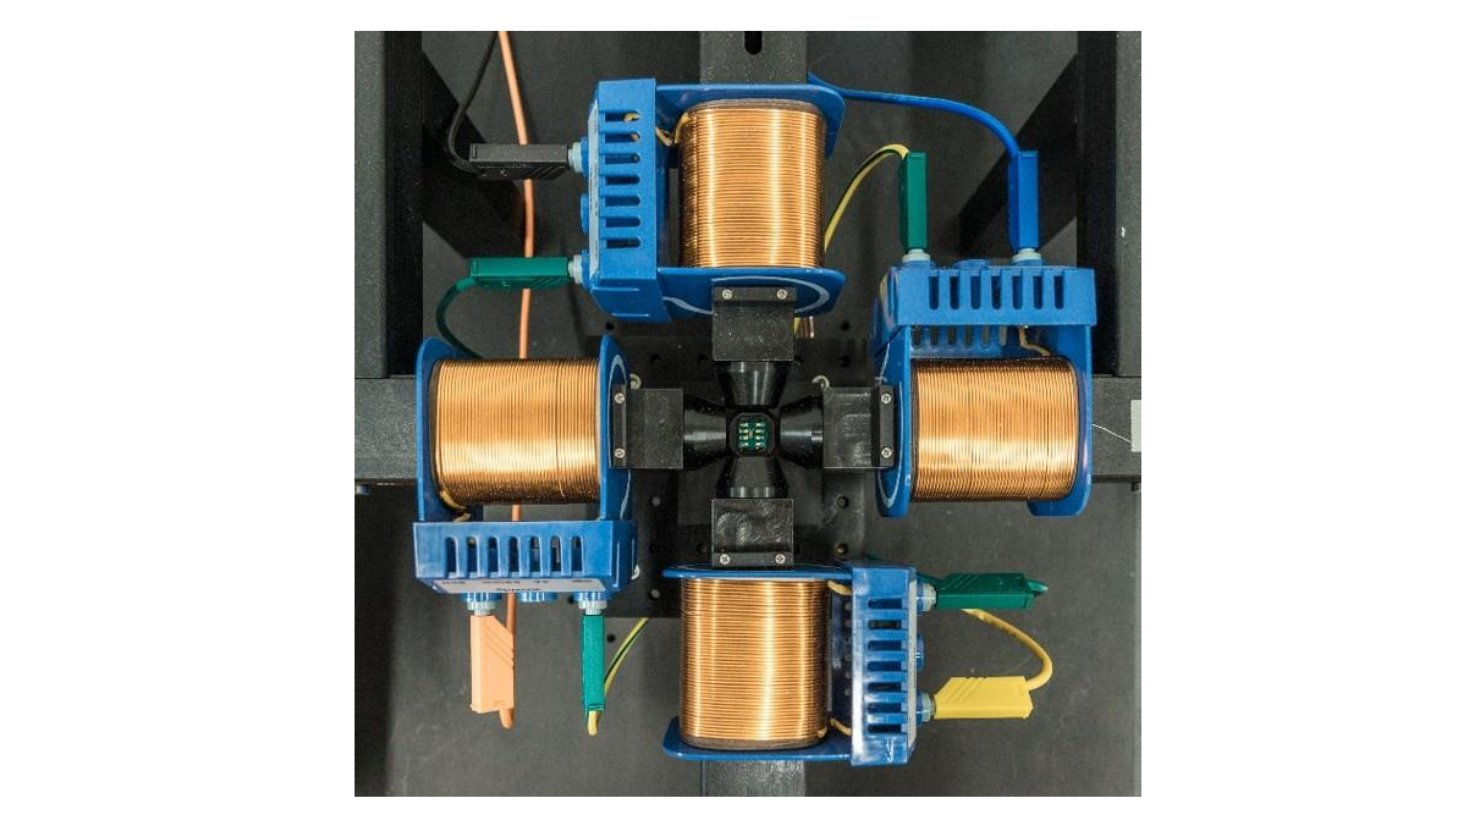
\includegraphics[width=\textwidth]{Versuchsaufbau.jpg}
\caption{Experimenteller Aufbau zur Messung des GMR- und des AMR-Effekts: In der Mitte befindet sich die Probe in einem Sockel. Die vier Spulen erzeugen ein annähernd homogenes Magnetfeld, dass längs jeder Richtung symmetrisch um den Wert \(B=0\) eingestellt werden kann.}
\end{figure} \\
Zwei sich gegenüberliegende Spulen erzeugen dabei jeweils ein antiparalleles Magnetfeld. Falls durch alle vier Spulen der gleiche Strom fließt, verschwindet daher das Magnetfeld im Zentrum, wo sich der Sockel mit Probe befindet. Fließen jedoch durch zwei gegenüberliegende Spulen verschiedene Ströme, ergibt sich ein resultierendes Feld, das in Richtung des stärkeren Feldes zeigt. Da die Maxwell-Gleichungen linear sind, überlagern sich die Felder in \(x\)- und \(y\)-Richtung störungsfrei, sodass man das Magnetfeld in beiden Richtungen symmetrisch durch den Wert \(B=0\) fahren kann. Will man längs der \(x\)-Richtung symmetrisch durch null fahren, lässt man eine der Spulen konstant auf  \(I_1^{(x)}=2 \ \mathrm{A}\) und variiert in der anderen Spule die Stromstärke \(I_2^{(x)} = 0\hdots 4 \ \mathrm{A}\). Die beiden Spulen in \(y\)-Richtung bleiben konstant auf \(I_1^{(y)} = I_2^{(y)} = 2 \ \mathrm{A}\). Durch den Übergang zu Polarkoordinaten ist es möglich, Formeln für die Reichweiten von \(x\) und \(y\) bei einem symmetrischen Durchlauf durch \(B=0\) längs einer beliebig gedrehten Achse zu ermitteln. Diese lauten:
\begin{align*}
x_{\mathrm{Start}} = 2 - 2\cos\vartheta \quad , \quad x_{\mathrm{End}} = 2 + 2\cos\vartheta \\
y_{\mathrm{Start}} = 2 - 2\sin\vartheta \quad , \quad y_{\mathrm{End}} = 2 + 2\sin\vartheta 
\end{align*}
Solche Intervalle für \(x\) und \(y\) wurden für verschiedene Winkel \(\vartheta\) berechnet: \\\\
\begin{table}[h!]
\centering
\begin{tabular}{|c|c|c|c|c|} \hline
$\vartheta / ^{\circ}$ & $x_{\text{start}}$/A & $x_{\text{end}}$/A & $y_{\text{start}}$/A & $y_{\text{end}}$/A \\\hline
0  & 0.00 & 4.00 & 2.00 & 2.00 \\\hline
15 & 0.07 & 3.93 & 1.48 & 2.52 \\\hline
30 & 0.27 & 3.73 & 1.00 & 3.00 \\\hline
45 & 0.59 & 3.41 & 0.59 & 3.41 \\\hline
60 & 1.00 & 3.00 & 0.27 & 3.73 \\\hline
75 & 1.48 & 2.52 & 0.07 & 3.93 \\\hline
90 & 2.00 & 2.00 & 0.00 & 4.00  \\\hline
\end{tabular}
%\caption{Verwendete Intervallgrenzen zur Erstellung der Sweeps für verschiedene Winkel \(\vartheta\)}
\end{table} \\\\
Anschließend wurdem mithilfe des Programms "matrixGui" \ Sweeps erstellt, also kleine Programme, die genau diese Intervalle in jeweils 101 Schritten durchlaufen. Die Sweeps wurden dann dem Messprogramm "matrixGui" übergeben, welches damit den Strom in den Spulen automatisch gemäß den Sweeps durchlaufen lässt und dabei die Messwerte aufnimmt. \\\\
Zusätzlich wurde eine Drehung simuliert, bei der Vektor \(\vec{B}\) der magnetischen Flussdichte betragsmäßig konstant bleibt, sich aber einmal im Bereich von \(0^{\circ}\) bis \(360^{\circ}\) dreht. Wenn \(\vartheta\) der Drehwinkel ist, kann man hierfür die Formeln für die Endwerte der Sweeps verwenden:
\begin{align*}
x(\vartheta) = 2 + 2\cos\vartheta \\
y(\vartheta) = 2 + 2\sin\vartheta 
\end{align*}
Wählt man diese Werte für den Strom der Spulen, ergibt sich eine magnetische Flussdichte \(\vec{B}\) von konstantem Betrag, die in Richtung des Einheitsvektors \(\vec{e}_r = \cos\vartheta \vec{e}_x + \sin\vartheta \vec{e}_y\) zeigt. Das Problem ist hierbei, dass das Messprogramm nur lineare Sweeps erzeugen konnte, die Sinus- und Cosinusfunktionen aber nichtlinear sind. Anstatt alle Werte einzeln einzugeben, haben wir die trigonometrischen Funktionen durch Sägezahnkurven angenähert, wie in folgender Abbildung dargestellt: 
\newpage
\begin{figure}[h!]\centering
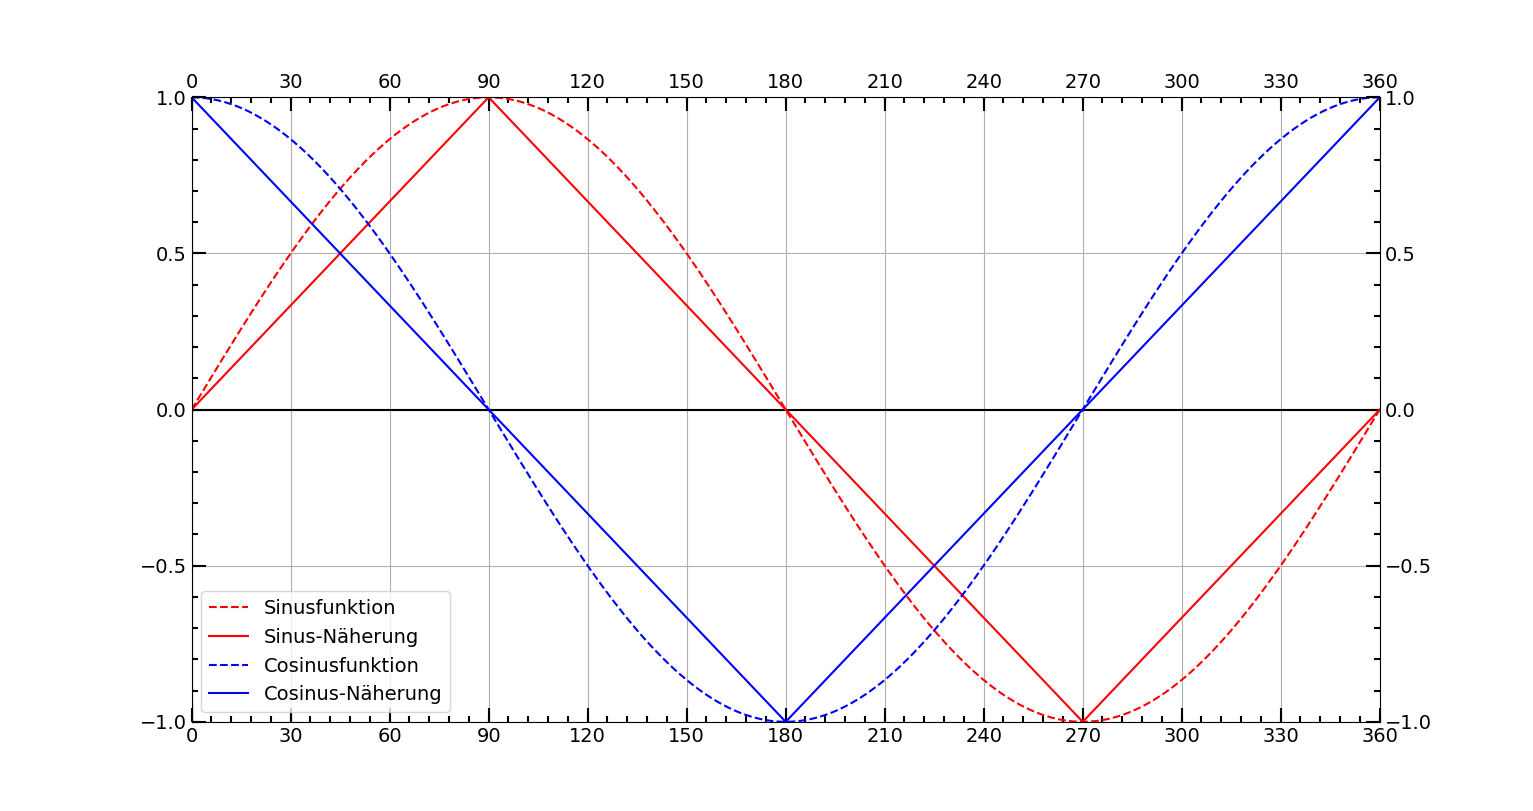
\includegraphics[width=\textwidth]{Sinus_und_Cosinus_Naeherung.png}
\caption{Näherung der trigonometrischen Funktionen durch Sägezahnkurven}
\end{figure} 
Die Sägezahnkurven lassen sich durch vier lineare Sweeps sehr einfach automatisch erstellen und bieten so zumindest eine gute Näherung für die praktisch nicht zugänglichen Sinus- und Cosinusfunktionen. Unter Berücksichtigung des Offsets und des Faktors 2 wurden dann folgende Sweeps generiert:
\begin{itemize}
\item 4 \(x\)-Sweeps zu jeweils 26 Werten, linear 
\begin{enumerate}
\item Sweep: \(x=4 \ \mathrm{A}\) bis \(x=2 \ \mathrm{A}\)
\item Sweep: \(x=2 \ \mathrm{A}\) bis \(x=0 \ \mathrm{A}\)
\item Sweep: \(x=0 \ \mathrm{A}\) bis \(x=2 \ \mathrm{A}\)
\item Sweep: \(x=2 \ \mathrm{A}\) bis \(x=4 \ \mathrm{A}\)
\end{enumerate}
\item 4 \(y\)-Sweeps zu jeweils 26 Werten, linear 
\begin{enumerate}
\item Sweep: \(y=2 \ \mathrm{A}\) bis \(y=4 \ \mathrm{A}\)
\item Sweep: \(y=4 \ \mathrm{A}\) bis \(y=2 \ \mathrm{A}\)
\item Sweep: \(y=2 \ \mathrm{A}\) bis \(y=0 \ \mathrm{A}\)
\item Sweep: \(y=0 \ \mathrm{A}\) bis \(y=2 \ \mathrm{A}\)
\end{enumerate}
\end{itemize}
Diese Sweeps wurden dann zu einem Gesamt-Sweep zusammengeführt und für die Simulation der Drehung verwendet. \\\\
Als nächstes wurde eine Messung an einer GMR-Probe durchgeführt, die uns ebenfalls fertig zur Verfügung gestellt wurde. Für diese wurde nur eine Messung für die Winkel \(\vartheta=0^{\circ}\) und \(\vartheta=90^{\circ}\) durchgeführt sowie eine Drehung simuliert. Dafür wurden die Sweeps, die bereits im Versuch zum Anisotropen Magnetwiderstand erstellt wurden, wieder verwendet. Die Datenauswertung erfolgte analog. \\\\
Da die eigentliche Messung vollautomatisch erfolgte und daher nicht so viel Zeit erforderte, wurde uns noch eine dritte, unbekannte Probe zusätzlich zu den regulär durchzuführenden Experimenten ausgehändigt. Für diese wurden mit denselben Sweeps Messungen für die Winkel \(\vartheta=0^{\circ},15^{\circ},30^{\circ},45^{\circ},60^{\circ},75^{\circ},90^{\circ}\) durchgeführt sowie abermals die Drehung simuliert. \\\\
Zum Abschluss des Versuches wurde noch ein kommerzielles elektronisches Bauelement untersucht. Dafür wurden Messungen bei \(\vartheta=0^{\circ}\) und \(\vartheta=90^{\circ}\) durchgeführt sowie eine Drehung simuliert. \\\\
Sämtliche so erhaltenen Daten wurden in digitaler Form gespeichert und später mit der Programmiersprache Python grafisch aufbereitet. Die dabei entstandenen Diagramme sind in der Auswertung dargestellt.
\section{Auswertung}
\subsection{Teil 1: Erzeugung und Quantifizierung von Magnetfeldern}
Für die verwendete Hall-Sonde wurde ein Umrechnungsfaktor von \(c = 3 \frac{\mathrm{mT}}{\Omega}\) von Widerstand zu Feld vorgegeben. Damit kann aus den gemessenen Daten jeweils das Magnetfeld ermittelt und mit der theoretischen Vorhersage für eine lange dünne Spule verglichen werden: \\\\
\underline{\underline{Luftspule:}} 
\begin{table}[h!]
\begin{tabular}{|c|c|c|c|c|} 
\hline
\(I/ \mathrm{A}\) & \(U / \mathrm{V}\) & \((R \pm \Delta R )/ \Omega\) & \((B_{\mathrm{exp}} \pm \Delta B_{\mathrm{exp}}) / \mathrm{mT}\) & \(B_{\mathrm{theor}}  / \mathrm{mT}\)\\\hline
1 & 1.69 & \( 1.480 \pm 0.015 \) & \( 4.440 \pm 0.045 \) & 5.800 \\\hline
2 & 3.39 & \( 2.955 \pm 0.015 \) & \( 8.865 \pm 0.045 \) & 11.600 \\\hline
3 & 5.09 & \( 4.428 \pm 0.015 \) & \( 13.284 \pm 0.045 \) & 17.400 \\\hline
4 & 6.66 & \( 5.892 \pm 0.015 \) & \( 17.676 \pm 0.045 \) & 23.199 \\\hline
\end{tabular}
\end{table} 
\newpage
\underline{\underline{Spule mit Eisenkern:}} 
\begin{table}[h!]
\begin{tabular}{|c|c|c|c|c|c|} 
\hline
\(I/ \mathrm{A}\) & \(U / \mathrm{V}\) & \((R \pm \Delta R )/ \Omega\) & \((B_{\mathrm{exp}} \pm \Delta B_{\mathrm{exp}}) / \mathrm{mT}\)  & \(B_{\mathrm{theor}}  / \mathrm{mT}\) \\\hline
1 & 1.66 & \( 16.537 \pm 0.015 \) & \( 49.611 \pm 0.045 \) & 83.368 \\\hline
2 & 3.32 & \( 36.170 \pm 0.015 \) & \( 108.510 \pm 0.045 \) & 166.737 \\\hline
3 & 5.01 & \( 57.676 \pm 0.015 \) & \( 173.028 \pm 0.045 \) & 250.105 \\\hline
4 & 6.70 & \( 79.116 \pm 0.015 \) & \( 237.348 \pm 0.045 \) & 333.474 \\\hline
\end{tabular}
\end{table} \\\\
Für beide experimentellen Werte wurde ein linearer Fit durchgeführt. Dabei ergaben sich folgende Parameter der Geraden:
\begin{align*}
\underline{\text{Luftspule:}} \quad m &= (4.413 \pm 0.005) \ \frac{\mathrm{mT}}{\mathrm{A}} \\
B_0 &= (0.035 \pm 0.015) \ \mathrm{mT} \\\\
\underline{\text{Spule mit Eisenkern:}}\quad m &= (62.8 \pm 1.0) \ \frac{\mathrm{mT}}{\mathrm{A}}\\
B_0 &= (-14.8 \pm 2.6) \ \mathrm{mT}
\end{align*}
Die Anstiege entsprechen gemäß
\[B = \underbrace{\mu_0\mu_{\mathrm{rel.}}\frac{N}{l}}_{:=m}\cdot I = m\cdot I\]
einem Faktor \(m= \mu_0\mu_{\mathrm{rel.}}\frac{N}{l}\), der die Geometrie der Spule und die Permeabilität des Füllmaterials enthält. Dividiert man die beiden Anstiege, so kürzen sich sämtliche Geometriefaktoren sowie die magnetische Feldkonstante heraus und es bleibt nur das Verhältnis von \(\mu_{\mathrm{Luft}}\) und \(\mu_{\mathrm{Eisen}}\) übrig:
\[\frac{m_{\mathrm{Eisen}}}{m_{\mathrm{Luft}}} = \frac{\mu_0\mu_{\mathrm{Eisen}}\frac{N}{l}}{\mu_0\mu_{\mathrm{Luft}}\frac{N}{l}} = \frac{\mu_{\mathrm{Eisen}}}{\mu_{\mathrm{Luft}}} \approx \mu_{\mathrm{Eisen}}\]
weil die Permeabilität von Luft in sehr guter Näherung gleich eins ist. Mit den ermittelten Anstiegen erhält man:
\[\mu_{\mathrm{Eisen}} = \frac{62.772 \ \frac{\mathrm{mT}}{\mathrm{A}}}{4.412 \ \frac{\mathrm{mT}}{\mathrm{A}}} = 14.225\]
Mit dieser Permeabilität wurden dann gemäß \(B = \mu_0\mu_{\mathrm{rel.}}\frac{N}{l}\cdot I \) die theoretischen Werte in der zweiten Tabelle ausgerechnet. Diese enthalten zwar den experimentell ermittelten Wert für \(\mu_{\mathrm{Fe}}\), geben aber den theoretisch zu erwartenden linearen Zusammenhang zwischen \(B\) und \(I\) wieder. Die Unsicherheit der Permeabilität folgt aus der Gauß'schen Fehlerfortpflanzung:
\begin{align*}
\Delta\mu = \sqrt{\left(\frac{\partial\mu_{\mathrm{Eisen}}}{\partial m_{\mathrm{Eisen}}}\right)^2 + \left(\frac{\partial\mu_{\mathrm{Eisen}}}{\partial m_{\mathrm{Luft}}}\right)^2} = \sqrt{\left(\frac{\Delta m_{\mathrm{Eisen}}}{m_{\mathrm{Luft}}}\right)^2 + \left( - \frac{m_{\mathrm{Eisen}}\Delta m_{\mathrm{Luft}}}{m_{\mathrm{Luft}}^2}\right)^2} = 3.356
\end{align*}
Damit ergibt sich für die relative Permeabilität des Eisens:
\[\underline{\underline{\mu_{\mathrm{Eisen}} = (14.2 \pm 3.4)}}\]
Aus der Unsicherheit der Permeabilität folgt dann auch ein Toleranzbereich für die theoretische Vorhersage, da in diese ja der erst zu ermittelnde und daher unsichere Wert \(\mu\) eingeht:
\[m_{\mathrm{theor}} = \mu_0\mu_{\mathrm{Eisen}}\frac{N}{l} \quad\Longrightarrow\quad \Delta m_{\mathrm{theor}} = \mu_0\Delta\mu_{\mathrm{Eisen}}\frac{N}{l} = 19.5 \frac{\mathrm{mT}}{\mathrm{A}}\]
In der folgenden Abbildung sind die experimentellen Messwerte und die theoretische Vorhersage für beide Fälle inklusive der Parameter dargestellt: \\\\
\begin{figure}[h!]\centering
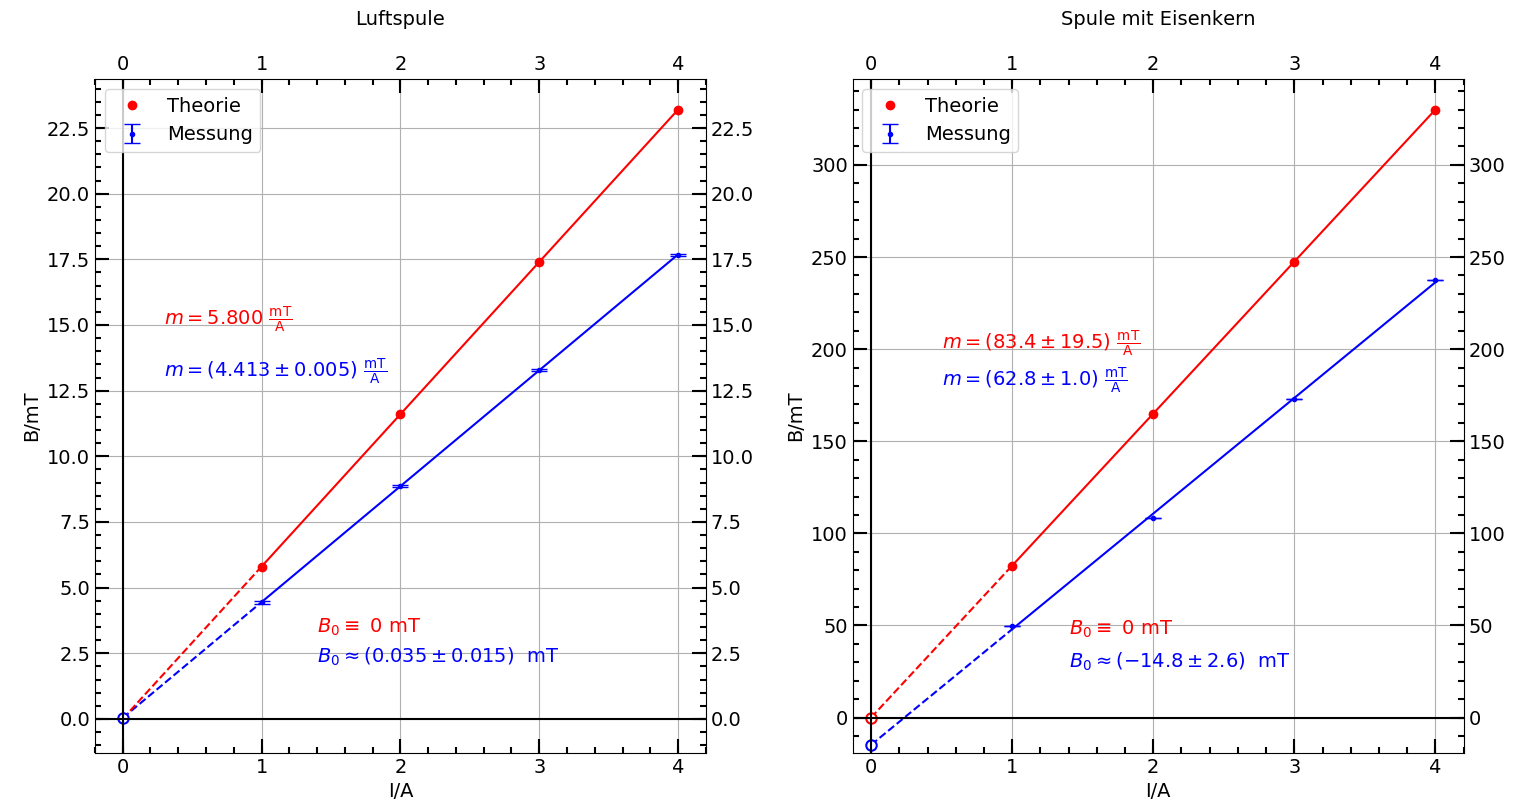
\includegraphics[width=\textwidth]{Hall_Sonde.png}
\caption{Messungen der magnetischen Flussdichte mit einer Hallsonde für eine Luftspule und eine Spule mit Eisenkern zur Bestimmung der Permeabilität des Eisens; Vergleich von Theorie und Experiment}
\end{figure}  \\
Bei der Luftspule wird der zu erwartende lineare Zusammenhang sehr gut erfüllt; der extrapolierte Wert \(B_0\) ist sehr nahe bei null. Abweichungen gibt es im Anstieg. Das könnte einerseits an der potentiellen Verkippung der Hall-Sonde liegen, andererseits gibt es noch eine ganz andere Ursache: Die Spule muss konstruktionsbedingt einen Luftspalt haben, in den die Hallsonde eingeführt wird. Dadurch gibt es aber prinzipiell eine nicht zu vermeidende Feldstreuung, weil die magnetische Flussdichte im Bereich des Luftspaltes nicht mehr homogen ist. Es ist also zu erwarten, dass die tatsächlich gemessene Flussdichte immer unterhalb der theoretisch berechneten liegt. Die experimentellen Daten spiegeln diesen Befund wieder. \\\\
Größere Abweichungen bestehen bei der Spule mit Eisenkern. Auch hier ist der Anstieg bei den realen Messdaten kleiner als bei der theoretischen Berechnung, was an der Feldstreuung liegt. Obwohl die gemessenen Werte sehr gut auf einer Geraden liegen, gilt trotzdem nur ein affin-linearer Zusammenhang, weil der extrapolierte Wert \(B_0 = (-14.8 \pm 2.6) \ \mathrm{mT}\) signifikant von null verschieden ist. Eine Erklärung hierfür ist, dass Eisen ein ferromagnetisches Material ist: Da der Versuch bereits von vielen anderen Gruppen durchgeführt wurde, ist es durchaus denkbar, dass der Eisenkern bereits eine nicht-verschwindende Magnetisierung hat, die sich in der Messung bemerkbar macht. \\\\
Insgesamt kann man sagen, dass die direkte Proportionalität zwischen magnetischer Flussdichte und Stromstärke sehr gut bestätigt werden konnte. Es gibt zwar messbare Abweichungen von theoretischen Werten; diese lassen sich aber schlüssig begründen.
\subsection{Probe 1:}
Für die erste Probe wurden Messungen für sieben verschiedene Winkel vorgenommen sowie ein Drehung simuliert. Bei der Winkelmessung wurde jeweils der elektrische Widerstand in Abhängigkeit vom Magnetfeld dargestellt. Für \(\vartheta\neq 0^{\circ},90^{\circ}\) ist in jedem Diagramm jeweils die Abhängigkeit in \(x\)- und \(y\)-Richtung für einen festen Winkel dargestellt. Da bei den Messungen längs der Koordinatenachsen (\(\vartheta = 0^{\circ},90^{\circ}\)) das Feld nur in einer Richtung variiert wird, gibt es hier für jeden Winkel nur ein Diagramm. Hier wurden daher die Messungen für  \(\vartheta = 0^{\circ}\) und \(\vartheta = 90^{\circ}\) gegenübergestellt. Die Winkelmessungen ergaben:
\newpage
\begin{figure}[h!]\centering
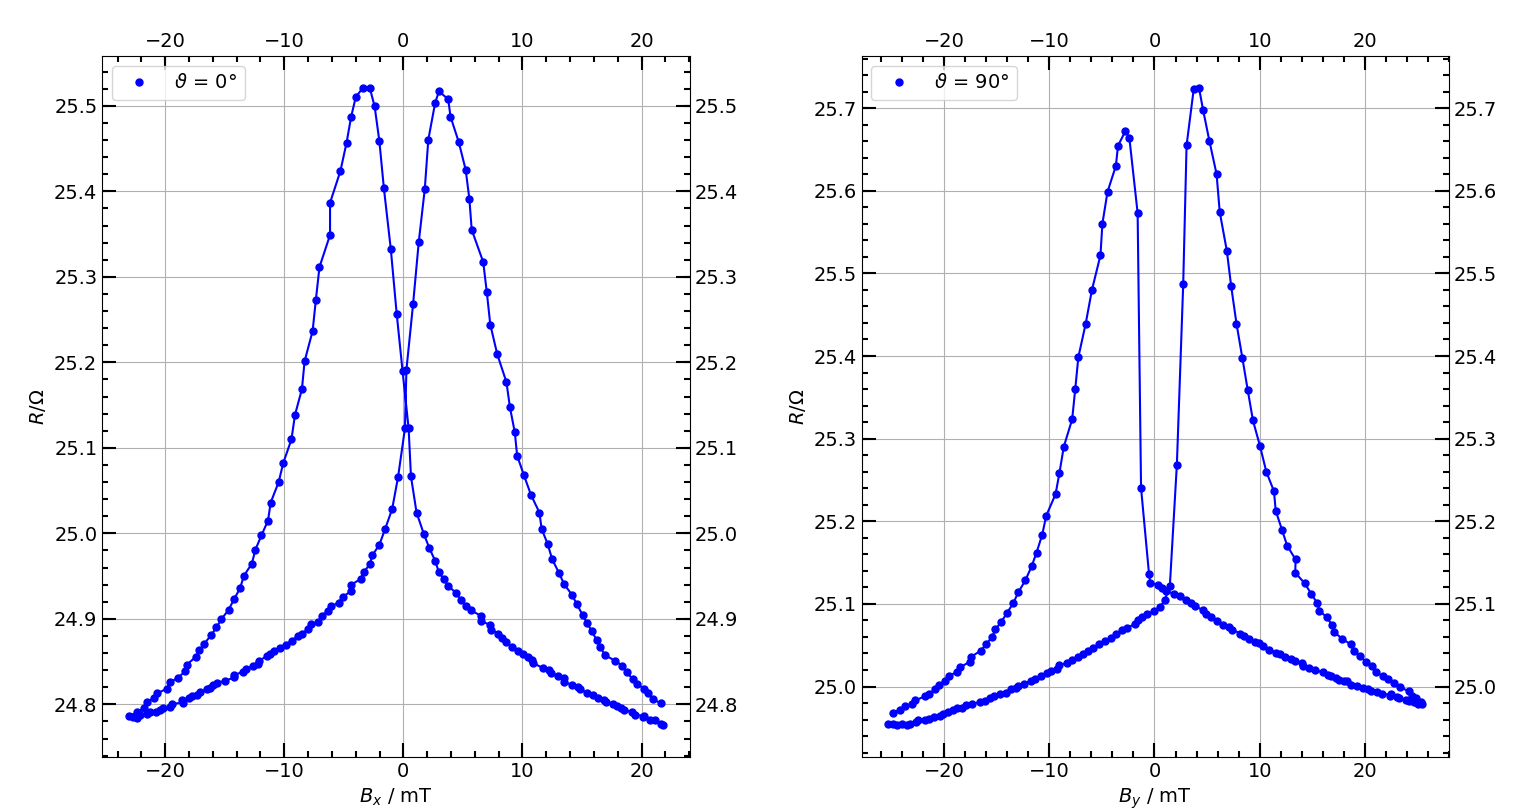
\includegraphics[width=\textwidth]{Probe1_0_und_90_Grad.png}
\caption{Probe 1: Messungen für \(\vartheta=0^{\circ}\) (\(x\)-Richtung) und \(\vartheta=90^{\circ}\) (\(y\)-Richtung)}
\end{figure} 
\begin{figure}[h!]\centering
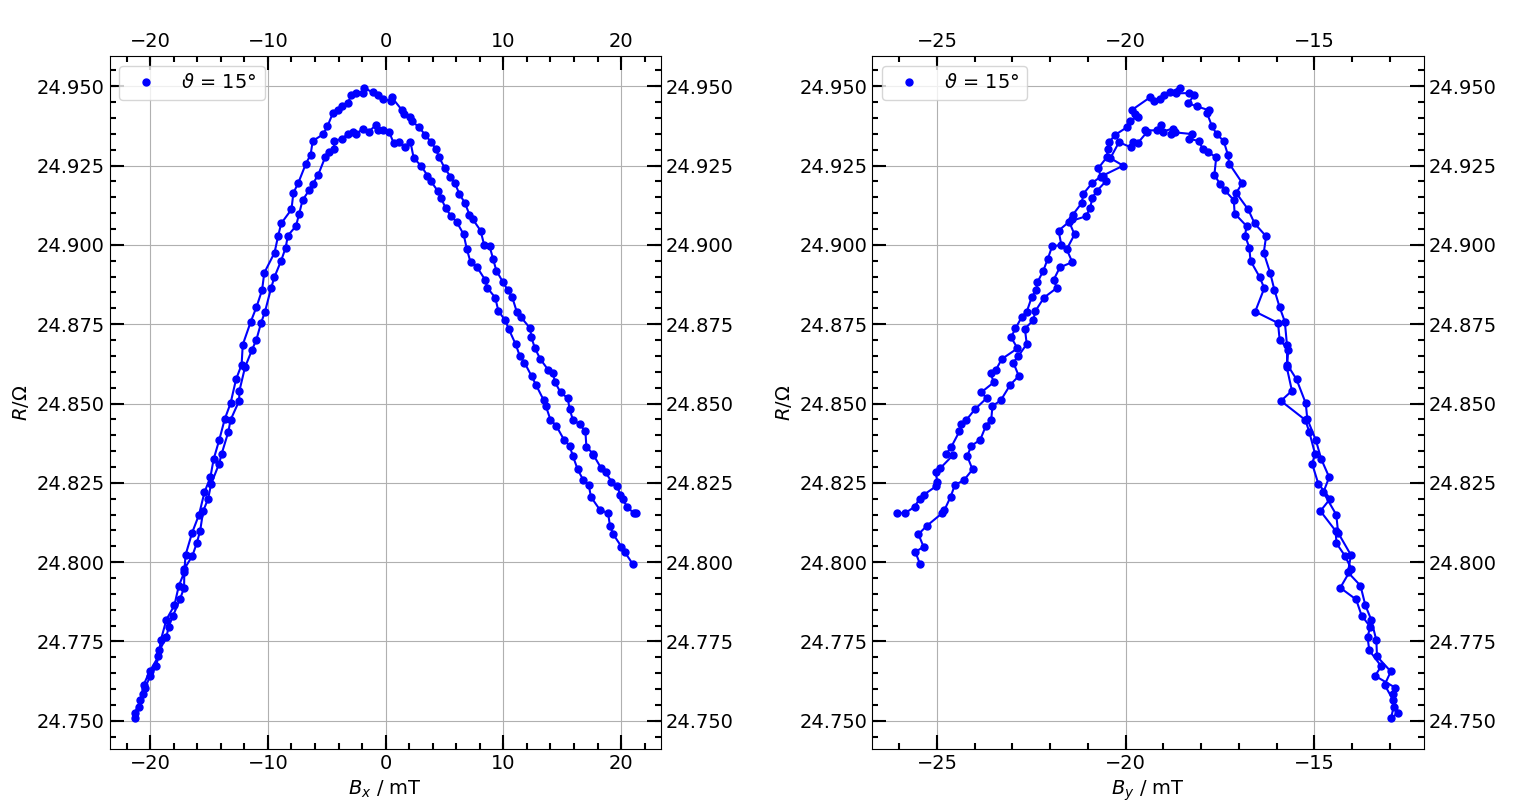
\includegraphics[width=\textwidth]{Probe1_15_Grad.png}
\caption{Probe 1: Messung für \(\vartheta=15^{\circ}\), Abhängigkeiten von den \(x\)- und \(y\)-Komponenten von \(B\)}
\end{figure} 
\newpage
\begin{figure}[h!]\centering
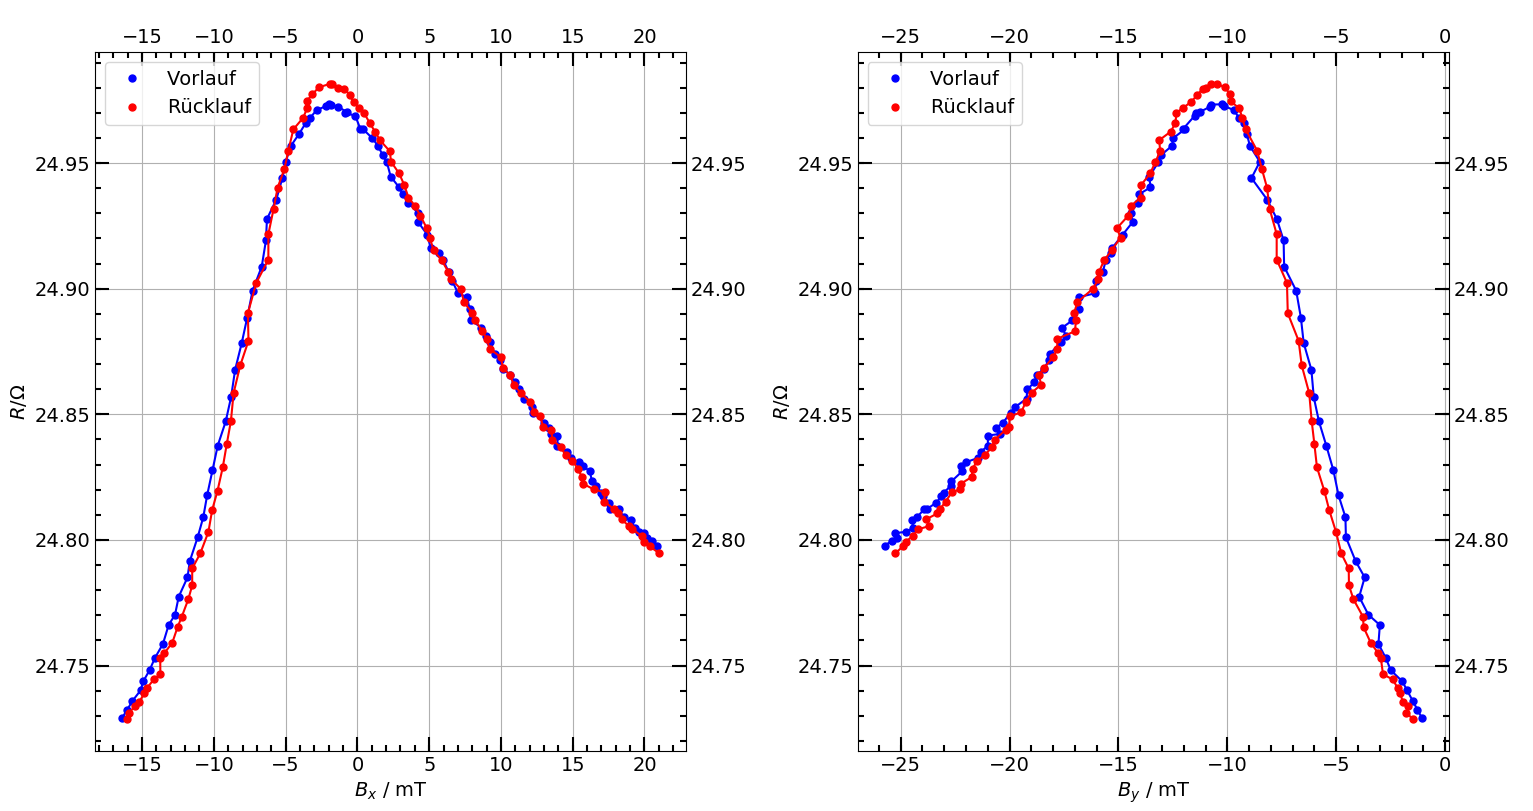
\includegraphics[width=\textwidth]{Probe1_30_Grad.png}
\caption{Probe 1: Messung für \(\vartheta=30^{\circ}\), Abhängigkeiten von den \(x\)- und \(y\)-Komponenten von \(B\)}
\end{figure} 
\begin{figure}[h!]\centering
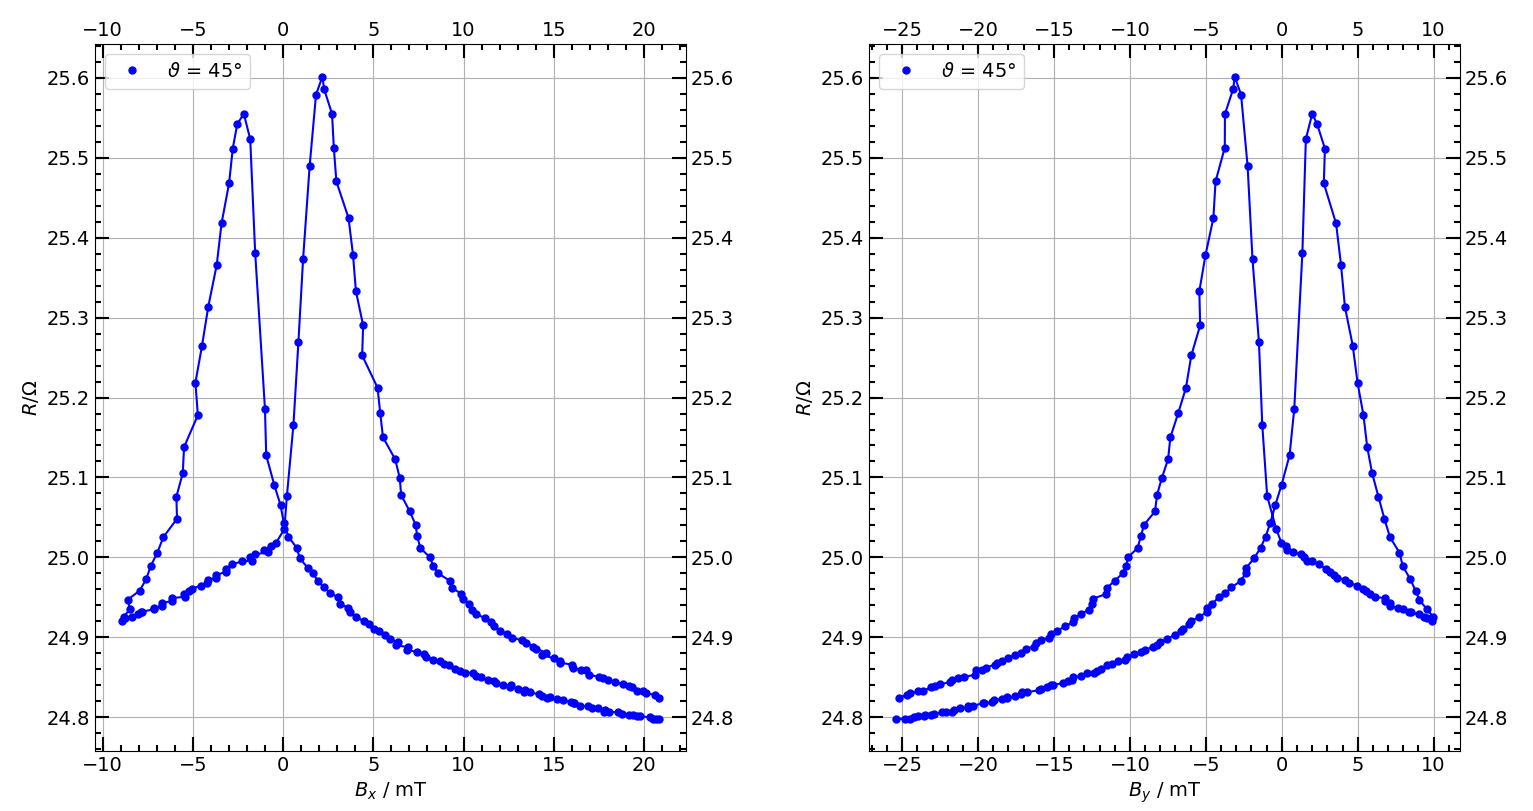
\includegraphics[width=\textwidth]{Probe1_45_Grad.png}
\caption{Probe 1: Messung für \(\vartheta=45^{\circ}\), Abhängigkeiten von den \(x\)- und \(y\)-Komponenten von \(B\)}
\end{figure} 
\newpage
\begin{figure}[h!]\centering
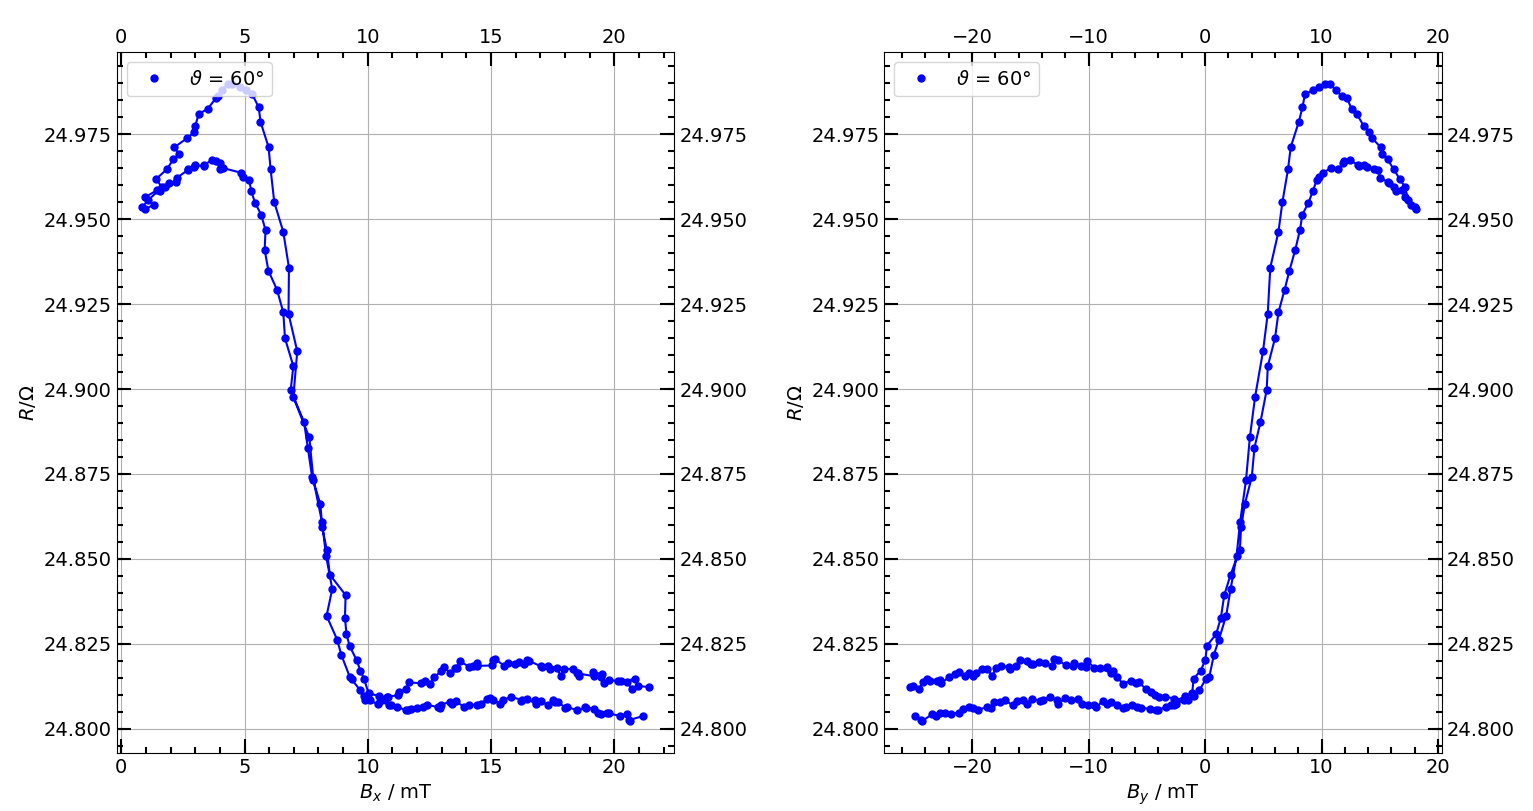
\includegraphics[width=\textwidth]{Probe1_60_Grad.png}
\caption{Probe 1: Messung für \(\vartheta=60^{\circ}\), Abhängigkeiten von den \(x\)- und \(y\)-Komponenten von \(B\)}
\end{figure} 
\begin{figure}[h!]\centering
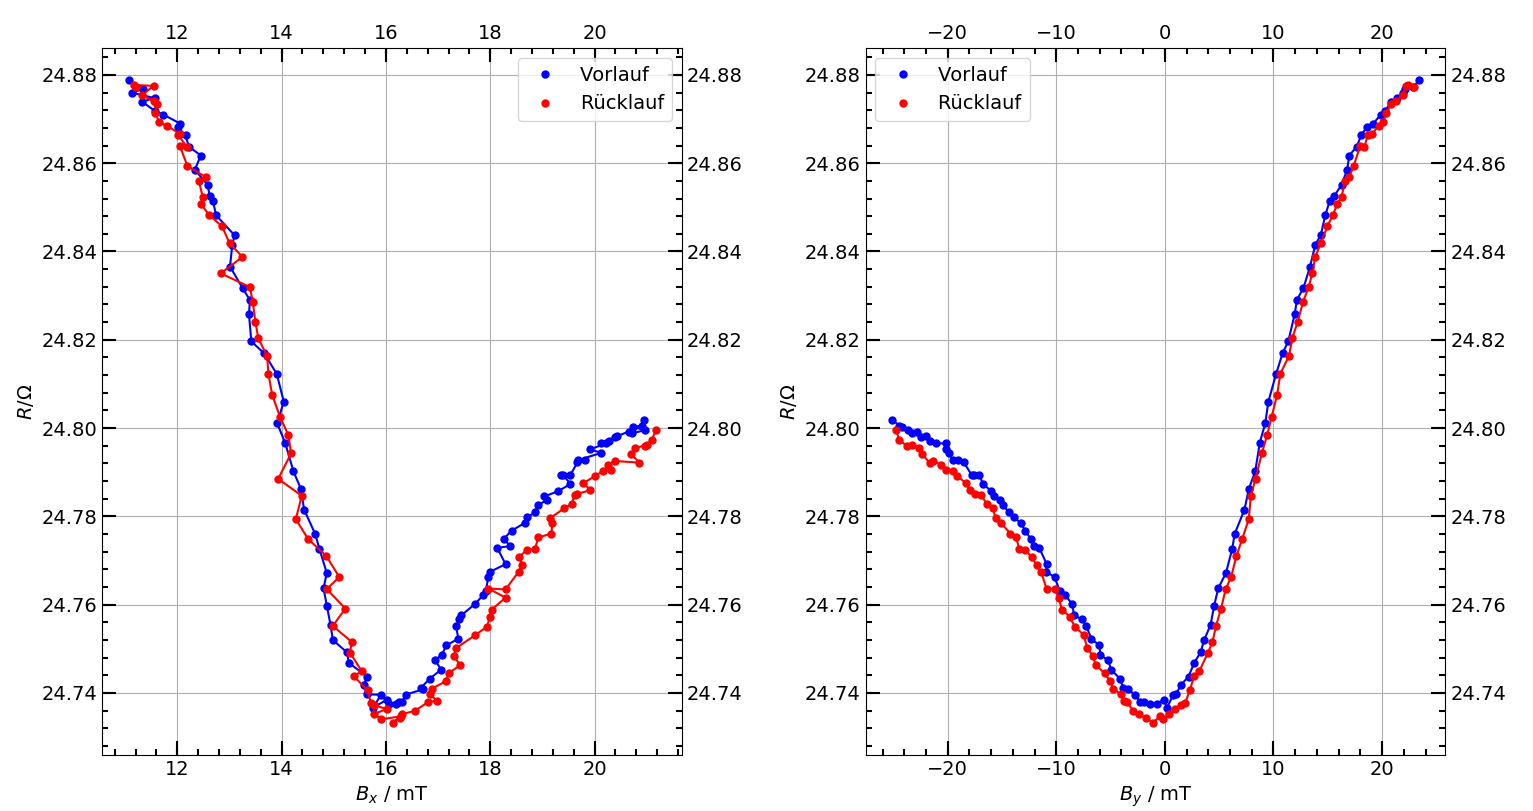
\includegraphics[width=\textwidth]{Probe1_75_Grad.png}
\caption{Probe 1: Messung für \(\vartheta=75^{\circ}\), Abhängigkeiten von den \(x\)- und \(y\)-Komponenten von \(B\)}
\end{figure}
\newpage  
Hier geht es weiter.
Bei der Simulation der Drehung wurde nach Programmierung des Sweeps der elektrische Widerstand als Funktion der Zeit gemessen. Die \(t_{\mathrm{Start}}\) und \(t_{\mathrm{End}}\) den Winkeln \(\vartheta = 0^{\circ}\) und \(\vartheta = 360^{\circ}\) entsprechen, kann man die Messzeit in Winkel umrechnen. Es sind beide Zusammenhänge dargestellt: \\\\
\begin{figure}[h!]\centering
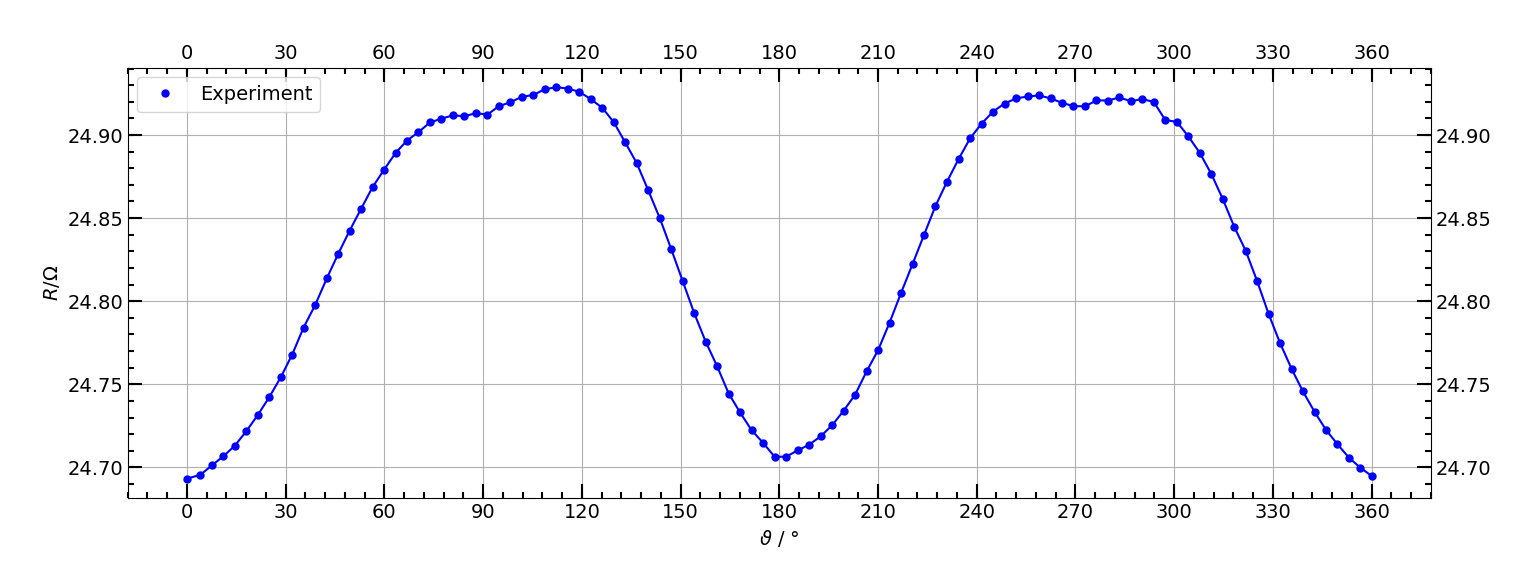
\includegraphics[width=\textwidth]{Probe1_Drehung.png}
\caption{Probe 1: Simulation einer vollen Drehung durch lineare Sweeps}
\end{figure}\\
Hier geht es wieder weiter.
 % Bibliographie/Literaturverzeichnis
%    \begin{thebibliography}{9}
%    \bibitem{gitterfehler}
%    \emph{Gitterfehler},
%%    \url{https://de.wikipedia.org/wiki/Gitterfehler#Nulldimensionale_Gitterfehler},
 %   9.\,Dez.~2019.
 %   \bibitem{wiki:Praktischer_Strahlenschutz}
 %   \emph{Schematische Darstellung von Stufenversetzungen (2D)},
 %   \url{https://de.wikipedia.org/wiki/Versetzung_(Materialwissenschaft)#/media/Datei:Versetzung_im_2D-Kristall.svg},
 %   12.\,Dez.~2019.
 %\bibitem{gitterfehler}
 %   \emph{Schematische Darstellung von Stufenversetzungen (3D)},
 %%   \url{https://de.wikipedia.org/wiki/Versetzung_(Materialwissenschaft)#/media/Datei:Dislocation_edge_d2.svgr},
  %  12.\,Dez.~2019.
%\bibitem{gitterfehler}
 %   \emph{Schematische Darstellung von Klein- bzw- Großwinkelkorngrenzen},
 %   \url{https://docplayer.org/71200148-Technische-universitaet-graz.html},
 %   12.\,Dez.~2019.
 %   \end{thebibliography}
%
% ----- BEISPIELTEXT ENDE -----
\end{document}